\documentclass[11pt,a4paper, notitlepage]{report}
\pdfoutput=1
%vons grund
\usepackage[T1]{fontenc}
\usepackage[utf8]{inputenc}
\usepackage[english, swedish]{babel} %OBS! Se till att vi får rätt språk.
\usepackage{amsmath}
\usepackage{lmodern}
\usepackage{units}
\usepackage{icomma}
\usepackage{color}
\usepackage{graphicx}
\graphicspath{ {bilder/} } %Gör så att man kan lägga alla bilder i en egen katalog
\usepackage{bbm}
\newcommand{\N}{\ensuremath{\mathbbm{N}}}
\newcommand{\Z}{\ensuremath{\mathbbm{Z}}}
\newcommand{\Q}{\ensuremath{\mathbbm{Q}}}
\newcommand{\R}{\ensuremath{\mathbbm{R}}}
\newcommand{\C}{\ensuremath{\mathbbm{C}}}
\newcommand{\rd}{\ensuremath{\mathrm{d}}}
\newcommand{\id}{\ensuremath{\,\rd}}
\usepackage{hyperref}

%%%%%%%%%%%%%%%%%%%%%%%Egna tillägg%%%%%%%%%%%%%%%%%%%%%%%
%%För att få referenser 'på svenska'
\usepackage[fixlanguage]{babelbib}
%\selectbiblanguage{swedish}
%\renewcommand\btxauthorcolon{:}
%%För att figurtext i underfigurer
\usepackage{subfigure} 
%%För att kunna inkludera andra PDF-dokument
\usepackage{pdfpages}
%%För att kunna ha roterade bilder
\usepackage{rotating}
%%För att kunna byta uppräkningsvisare t.ex. [label=\alph*)]
\usepackage{enumitem}
%%För att kunna lägga till 'bilagor' utan sidnumrering.
\usepackage{tocstyle}
\usetocstyle{standard}%För att få en vanlig TOC
                %no page numbers for part
\settocstylefeature[-1]{pagenumberbox}{\csname @gobble\endcsname}
\usepackage[nottoc]{tocbibind} %Puts an 'Reference' entry in the ToC.
%%För att kunna använda bra och ket
\usepackage{physics} %\bra{}\ket{} eller \expval{H}{\psi}
%%För att kunna rita snygga matriser
\usepackage{mathtools} %\begin{pmatrix*}[r] ... \end
%%För att kunna kommentera ut större stycken
%%Drar in tabell och figurtexter
\usepackage[margin=10 pt]{caption}
\usepackage{comment} %\begin{comment}
%%För att lägga in 'att göra'-noteringar i texten
\usepackage{todonotes} %\todo{...}, \todolist



%%För att inkludera MATLABkod. 
%%OBS: mcode är ett separat paket och man måste ha mcode.sty i samma
%%katalog som dokumentet.
%\usepackage[framed,numbered,autolinebreaks,useliterate]{mcode}
%\usepackage{listings} 
%\lstloadlanguages{matlab} 
%\lstset{language=matlab} 
%\lstset{literate= {å}{{\r{a}}}1 {ä}{{\"a}}1 {ö}{{\"o}}1 {Å}{{\r{A}}}1
%  {Ä}{{\"A}}1 {Ö}{{\"O}}1}%För att få svenska bokstäver från MATLAB.


%%%%%%%%%%%%%%%%%%%%%%%Formatering%%%%%%%%%%%%%%%%%%%%%%%%
%%Partiell derivata
\newcommand{\pd}{\ensuremath{\partial}}
%%Följer ISO-8601 oberoende av språk.
\usepackage[iso, swedish]{isodate}
%%Göra grader Celcius
\newcommand{\degC}{\ifmmode \,^\circ\mathrm{C} \else $\,^\circ\mathrm{C}$ \fi}
%%Figurreferenser
\newcommand{\figref}{\figurename~\ref} 
%%Tabellreferenser
\newcommand{\tabref}{\tablename~\ref} %Stor bokstav i början

%%Det ska vara ett rakt µ i prefixet
\usepackage{upgreek}
\newcommand{\micro}{\upmu}
%%Ohm enhetskommando
\newcommand{\ohm}{\ifmmode \Upomega \else $\Upomega$ \fi}

%%'e' och 'i' ska vara upprätt
\newcommand{\e}{\mathrm{e}}
\newcommand{\ii}{\mathrm{i}}

%%För att själv bestämma marginalerna. 
\usepackage[
%            top    = 3cm,
%            bottom = 3cm,
%            left   = 3cm, right  = 3cm
]{geometry}





\begin{document}

%Alla inledande sidor finns i 'titlepages.tex'.
\renewcommand{\thefootnote}{\fnsymbol{footnote}}

%kortkommandon för mailaddresserna
\newcommand{\andsunds}{andsunds@student.chalmers.se}
\newcommand{\rigon}{rigon@student.chalmers.se}



\pagenumbering{roman} %%Romersk sidnumrering i början
\begin{titlepage}
\newgeometry{top=3cm, bottom=2cm}

\newcommand{\HRule}{\rule{\linewidth}{0.5mm}} % Defines a new command for the horizontal lines, change thickness here

\center % Center everything on the page
 
%------------------------------------------------------------------------------------
%	HEADING SECTIONS
%------------------------------------------------------------------------------------

\textsc{\huge Chalmers tekniska högskola}\\[1.5cm] % Name of university/college
\textsc{\Large Rapport, Experimentell fysik 2}\\[0.2cm] % Major heading such as course name
\textsc{\large Termodynamik -- Uppgift 3 }\\[0.5cm] % Minor heading such as course title

%------------------------------------------------------------------------------------
%	TITLE SECTION
%------------------------------------------------------------------------------------

\HRule \\[0.4cm]
{ \LARGE \bfseries 
Studier av kvicksilveratomens atomära emissionsspektra samt absorptionsspektra av laserfärgämnena Rhodamin B och Kumarin 307
}\\[0.4cm] % Title of  document
\HRule \\[1.5cm]
 
%------------------------------------------------------------------------------------
%	AUTHOR SECTION
%------------------------------------------------------------------------------------

\begin{minipage}{0.4\textwidth}
\begin{flushleft} \large
\emph{Författare:}\\
Andréas Sundström\footnotemark{} \\
Rigon Demisai\footnotemark{} 
\end{flushleft}
\end{minipage}
~
\begin{minipage}{0.4\textwidth}
\begin{flushright} \large
\emph{Labassistent:} \\
Martin Wersäll
\end{flushright}
\end{minipage}\\[3cm]

\setcounter{footnote}{0}
\stepcounter{footnote}
  \footnotetext{\href{mailto:\andsunds}{\texttt{\andsunds}}}
\stepcounter{footnote}
  \footnotetext{\href{mailto:\rigon}{\texttt{\rigon}}}



%------------------------------------------------------------------------------------
%	DATE SECTION
%------------------------------------------------------------------------------------
% Följer ISO-standarden för tidsintervall:
% https://en.wikipedia.org/wiki/ISO_8601#Time_intervals
% "Double hyphen" också ok istället för '/'. -- i LaTeX är dock lite på gränsen
{ \large
\begin{tabular}{rc}
    Laboration utförd: & 2015-12-11/15 \\[0.1cm]
    Rapport inlämnad: & \today
\end{tabular}\\[1cm]
}

%------------------------------------------------------------------------------------
%	LOGO SECTION
%------------------------------------------------------------------------------------


\includegraphics[height=5cm]{logo.pdf} % Include a department/university logo
 
%------------------------------------------------------------------------------------

\vfill % Fill the rest of the page with whitespace

\end{titlepage}
\restoregeometry


\setcounter{page}{2}%detta är ANDRA (2) sidan

\renewcommand{\abstractname}{Sammandrag}
\begin{abstract}
Den här rapporten beskriver en spektroskopisk studie av
kvicksilveratomens atomära emissionsspektrum samt en studie av
laserfärgämnena rhodamin~B och kumarin~307 och deras
absorptionsspektra.
Ur emisionspektrumet från Hg har vissa av atomens energinivåer kartlagts,
baserat på kvanmekaniska regler och jämförelse med tidigare data på
Hg.  Kvicksilvrets emissionsspektra
är taget i intervallet 350--1100\,nm, där detekterades totalt 23
emissionstoppar, varefter 13 övergångar kunde identifieras.
Absorptionsspektrumen för rhodamin~B och kumarin~307 visar breda
absorptionsband vilket är kännetecknande för flourescerande ämnen som
består av stora organiska molekyler. 
Mätningarna har utförts med en Spex~270M spektrometer och
datainsamlingen har gjorts i LabView.
\end{abstract}

\renewcommand{\abstractname}{Abstract}
\begin{abstract}
This report describes a spectroscopic study of the atomic emision
spectrum of mercury, and also a study of the laser dyes Rhodamine~D
and Coumarin~307 and their absorption spectrum.
Som of the energylevels of Hg have been idetified from the emission
spectrum, based on quantum mecanichal rules and comparison with erlier
data on Hg. The emission spectrum of mercury was taken in the interval
of 350--1100\,nm, there a total of 23 emission lines were detected,
from which 13 different atomic transitions could be identified. 
The absorption spectrum of Rhodamin~B and Coumarin~307  show wide
absorption bands which are characteristic of big organic molecules.
THe measurements were made with a Spex~270M spectrometer and the data
collection was done through LabVIEW.
\end{abstract}

\clearpage
\renewcommand{\contentsname}{Innehållsförteckning}
\tableofcontents

\clearpage
\pagenumbering{arabic}
\setcounter{page}{1}

\renewcommand{\thefootnote}{\arabic{footnote}}
\setcounter{footnote}{0}


%Här ett exempel till på hur man använder input
\section{Exempel på \texttt{input}}
När man använder \texttt{input}-kommandot så betyder det bara att den stoppar in vad som står i den filen som man ger som input.

Det behövs inga andra konstigheter. Tänk bara på det som att man fortsätter skriver det man vill skriva, fast i en annan fil.



%%%%%%%%%%%%%%%%%%%%%% Här börjar huvudtexten %%%%%%%%%%%%%%%%%%%%%%
%\part{Inledning}

\chapter{Inledning}
\begin{itemize}
    \item Lite om transport i celler
    \item Resultat från dataanalysen
    \item Slutsatser vi kan dra från analysen
\end{itemize}


\section{Bakgrund}

Att partiklar kan ta sig fram genom cytoplasman spelar onekligen en viktig roll för många funktioner i cellen, exempelvis vid signaltransport när signalämnen tillåts sprida sig genom cellen. I vissa fall har hastigheten för spridning inte en betydande roll, men vid exempelvis celldelning är det viktigt att de delade cellerna får med sig en fullständig uppsättning organeller och en likvärdig blandning av cytoplasmans beståndsdelar. För detta krävs att beståndsdelarna kan förflytta sig runt och blandas.

I nuläget råder viss oenighet gällande hur cytoplasman, cellens fyllnadsmaterial, egentligen beter sig. Man har länge trott att cytoplasman kan ha två distinkta faser, en kolloid vätskefas med partiklar väl blandade i cytoplasman och en fas med komponenter i cellen som interagerar för att bilda ett sammanhängande nätverk som gör cytoplasman mer fast eller glasliknande.

Till en första approximation skulle rörelserna i cytoplasman kunna beskrivas med klassisk Brownsk rörelse där partiklarna krockar med mindre partiklar från omgivningen och där rörelsen kan beskrivas med en gaussisk propagator. Denna teori bygger dock på att man har termisk jämvikt och att partiklar rör sig i en helt viskös vätska, två kriterier som inte uppfylls i cytoplasman bland annat på grund av mitokondriernas energiutvinning. Andra modeller måste sålunda tillämpas för att nå en bättre beskrivning.

Tidigare studier på eukaryota celler har visat att partiklars rörlighet i cytoplasman beror på hur aktiv cellen är.\cite{Gou_etal2014} Rörligheten i de undersökta cellerna ökade trefaldigt om cellen drabbades av cancer jämfört med en normalt fungerande cell och den sammanlagda påverkan av motorproteinerna utpekas som en möjlig kandidat till fenomenet. Studier på bakterier har samtidigt visat att partiklarnas rörlighet minskade drastiskt om den metabola aktiviteten minskade. \cite{Parry_etal2014} Då bakterier saknar aktiv transport i sina celler försöker man här istället nå en förklaring via att cytoplasman blir mer vätskelik ju högre aktiviteten är och börjar likna mer ett elastiskt fast material då aktiviteten minskar men också att partiklarnas storlek spelar roll.

Datan som kommer analyseras under detta kandidatarbete utgörs av registrerade positioner för vissa utmarkerade proteinkluster i jästceller samt förhoppnigsvis av rörelsen för filament i cytoplasman. 

Jäst hör till riket svampar och utgörs av encelliga organismer. De är därmed varken djur, växter eller bakterier men delar vissa likheter med alla tre. Med sitt arvsanlag samlat i en cellkärna precis som djur- och växtceller skiljer sig jästceller från bakterier. De har även en vakuol och cellvägg som växtceller men saknar växtcellens kloroplaster. Att jästcellen är en encellig organism gör att den reproducerar sig snabbt vilket gör den smidig att arbeta med och vill man dra paralleller till djurceller uppvisar jästceller mer likheter med dessa än de likväl encelliga bakterierna. Djurcellernas komplicerade nät av proteintrådar som möjliggör en aktiv transport inom cellen finns inte hos jästceller som istället får förlita sig på passiv transport, förutom vid just celldelning. Med jästceller kan man därför undersöka om anomalier från klassisk Brownsk rörelse uppkommer även utan de stokastiska krafter som har sitt ursprung i motorproteinernas rörelse. Jästceller kan även gå i dvala där de intracellulära aktiviteterna minskar, vilket möjliggör undersökningar om huruvida cytoplasmans beståndsdelars rörlighet i cellen beror på cellens metabola tillstånd. \cite{Yeast}

Fördjupade studier av partikelrörelse i cellen skulle t ex kunna leda till mer effektiva läkemedel. Vet man hur transporten inom cellen sker underlättar det arbetet med att ta fram specialdesignad medicin.


\section{Syfte}

Syftet med detta kandidatarbete är att studera rörelser i celler och utifrån denna studie förhoppningsvis kunna ge en klarare bild av cytoplasmans betende. Detta ska framför allt ske genom att försöka ta fram en teoretisk förklaringsmodell för hur partiklar och filament (proteintrådar) rör sig genom cytoplasman. Denna modell är lämpligen en mikroskopisk beskrivning som ger upphov till en stokastisk modell. Ur en stokastisk modell kan sedan en makroskopisk, statistisk beskrivning uppnås och det är med denna statistiska beskrivning som modellen kan jämföras med data. 

Datan kommer från Max Planck Institutet i Dresden och utgörs av positionen för fluorescerande partiklar i jästceller. Partiklarna varierar i storlek vilket speglas av att de har olika stark ljusintensitet i mikroskopet. 
Vidare kommer förhoppningsvis även data från strängars rörelse i cytoplasman studeras. Tanken är att generalisera modellen för enskilda partiklars rörelse till att även kunna tillämpas för strängars rörelse.

%Syftet specificerar vad projektet är tänkt att resultera i och vilken typ av resultat som kommer att uppnås. Ett projekt kan ha flera syften som är relaterade till de ämnen/problem som presenteras i bakgrunden. I de flesta fall är det dock lämpligt att ha endast ett generellt syfte, som sedan bryts ner i mer detaljerade delar längre fram i rapporten/processen.

\section{Problem}

Målet med arbetet är att hitta en förklaringsmodell för hur partikar och förhoppningsvis filament rör sig med aktiv eller passiv transport i cellen och utifrån denna modell dra slutsatser om cytoplasmans natur. Dock är det inte säkert att datan från dessa filament kommer att finnas tillgänglig. Om så är fallet kommer arbetet begränsas till mindre, lokala partiklar för vilka data redan finns. Denna data består av tid-positionsdata för partiklar av storleksordning omkring 10--100\,nm uppmätta under jämna tidsintervall. %Med grund i tidigare studier gjorda på detta ämne ämnar vi leta efter liknande observationer och kanske hittar vi något nytt som vi kan tillföra till området.

\subsection{Dataanalys}

Ett första steg är att jämföra observationer på partiklar med motsvarande förutsägelser från teorin om Brownsk rörelse. Då det är känt att diffusionen i cytoplasman påverkas av motorprotein och man då funnit avvikelser\cite{Gou_etal2014} från klassisk Brownsk rörelse bör dessa redan funna avvikelser jämföras med den tillgängliga datan. I denna analys bör även skillnader mellan cellens olika stadier av metabol aktivitet kunna upptäckas. Vidare kan det vara intressant att undersöka hur partiklarna och filamenten borde bete sig om de endast utförde Brownsk rörelse i cytoplasman. Man kan då undersöka hur modellen påverkas om cytoplasman betraktas som en fluid vars beståndsdelar skiljer sig i storlek eller istället om den betraktas som ett elastiskt fast ämne. 
Härefter fås nu en grund varifrån man kan försöka hitta förklaringar till avvikelserna.

Men för att över huvud taget kunna analysera datan behöver man kunna veta osäkerheten i mätningarna. Detta är dock inte helt problemfritt då till exempel Brownsk rörelse i sig själv är en sorts brus. Brus brukar i vanliga fall hanteras genom att undersöka en sorts medelvärde. I det här fallet kommer datan från flera olika partiklar vilket gör att en direkt jämförelse av en undersökt parameter inte kan göras; man måste istället först finna ett samband mellan storleken på partiklarna och den parameter som man vill undersöka. 

I datan finns utöver position även en partikels intensitet i mikroskopet. Intensiteten beror med största sannolikhet på partikelns storlek; dock är det exakta sambandet inte helt klart vilket ger ännu en svårighet i hur datan ska analyseras. Troligen går det dock att från intensiteterna kunna jämföra olika partiklar och på så sätt ändå kunna utnyttja den i jämförelser mellan olika partiklar. 

\subsection{Teoretisk modell}

Från den observerade datan ska sedan en modell försöka konstrueras. Denna modell bör rimligtvis ta sin grund i frågorna:
\begin{itemize}
    \item Vad skulle en eventuell avvikelse från Brownsk rörelse kunna bero på?
    \item Är det den totala effekten av många motorprotein som arbetar oberoende av varandra som stör den annars kanske ideala slumpvandringen? 
    \item Beter sig cytoplasman olika vid olika tillfällen exempelvis beroende på vilken partikel den interagerar med? Ska cytoplasman betraktas som en fluid eller ett elastiskt fast ämne?
    \item Vad är det för egenskaper hos aktiva celler och celler i dvala som svarar mot de observerade skillnaderna mellan dem?
\end{itemize}

%Ska en del av detta stycke läggas som bakgrund?
Inspiration till hur modellen kan byggas upp kan hämtas från redan publicerade artiklar på området. En möjlig förklaringsmodell för anomal transport i celler utgörs av CTRW (continuous-time random walks). Här beskrivs rörelsemönstret med att partiklarna under majoriteten av tiden sitter bundna till olika strukturer för att sedan plötsligt ta sig vidare till en ny position efter en viss väntetid, där positionsändringen och väntetiden beskrivs av en stokastisk variabel. Anomal transport uppkommer här genom att medelväntetiden mellan två hopp blir oändlig och därmed att centrala-gränsvärdessatsen ej uppfylls. Summan av de stokastiska variablerna går således ej mot att bli normalfördelad, något som är grundläggande i teorin kring Brownsk rörelse.
En annan modell som kan undersökas är Fractional Brownian motion som bygger på superpositioner av Brownska processer med brus som uppvisar en beständig korrelation. Detta får transporten av partiklar att sakta ner med tiden jämfört med vanlig Brownsk rörelse. \cite{Hofling_Franosch}

För att testa dessa modellers riktighet för den mätdata som finns tillgänglig kan modellernas förutsägelser vad gäller bland annat autokorrelationsfunktioner samt mean square displacement testas. Finnes avvikelse kan modellen antingen avfärdas eller moduleras.
  
  
%Det här avsnittet är ofta den viktigaste delen av planeringsrapporten (och av den slutgiltiga rapporten). Den syftar till att identifiera frågan/frågorna som ska tas upp i projektet. Det är viktigt att gruppen gör en problem(uppgifts)analys även om det i projektförslaget redan finns ett problem (en uppgift) specificerat. Anledningen till detta är att det riktiga primära problemet ofta skiljer sig från det i början av uppdragsgivaren/förslagsställaren/kunden föreslagna. Problemanalysen syftar också till att bryta ner problemet/uppgiften i mindre och mer detaljerade delproblem/deluppgifter, vilket också leder till formulering av delsyften. Genom att göra detta får studenterna mycket bättre förståelse för de olika aspekterna av problemet/uppgiften. Utan den här information är det omöjligt att identifiera vilken information som behövs, vilka informationskällor som behövs,  och lämpliga tillvägagångssätt.

%En bra problemanalys som identifierar delproblem/deluppgifter och delsyften vilar i många fall på användning av teorier och modeller från litteraturen. En litteraturgenomgång bör därför genomföras tidigt i processen. 

\section{Avgränsningar}

Detta arbete kommer framförallt att fokusera på att analysera redan framtagen data för partiklars rörelse i cytoplasman och utifrån dessa observationer bygga en teoretisk modell med grund i redan föreslagna modeller. 

Att avbilda filament innebär stora svårigheter vilket har försvårat analysen av dess egenskaper och i dagsläget finns ingen fullkomlig modell som beskriver filamentens rörelse. Den teoretiska modellen som tas fram under kandidatarbetet kommer rimligtvis tas fram under vissa antaganden som begränsar dess användningsområde. Exempelvis kan variationer som uppstår vid betraktande av rörelser under olika tidsskalor komma att leda till svårigheter, bland annat i att finna en teoretisk modell som korrekt beskriver rörelsen oberoende av tidsskala. Således anses det mer rimligt att modellera rörelsen under antagandet att modellen i första hand beskriver rörelser för en viss tidsskala, förslagsvis observationer som varar i intervallet $\unit[10]{ms}$ till $\unit[10]{s}$ vilket speglar den data som hittills analyserats av gruppen.

Den datan som finns tillgänglig för analys består av datan från genmodifierade jästceller och den teoretiska modellen jämförs huvudsakligen med rörelse från dessa celler. Möjligheten att jämföra modellen med dels samma celler men med andra förutsättningar och dels med andra sorts celler kommer troligtvis vara något begränsad. 

Jästcellerna som har observerats saknar aktiv transport i stadier mellan celldelning, under vilka datan inhämtats. Därmed kan vi inte bekräfta en eventuell modell för celler med aktiv transport så som djur- och växtceller. En avgränsning i arbetet kan därför vara att inte fokusera på rörelse som beror på den sammanlagda effekten av motorproteiners bidrag till den aktiva transporten.



%\part{Huvuddel}

\chapter{Partikelrörelse i celler}


Bakgrund teori om cellen
\begin{itemize}
    \item Cytoplasmans uppbyggnad och struktur
    \item Brownsk rörelse, CTRW, Fractional Brownian motion
    \item Metabola tillståndets påverkan på partikelrörelsen
\end{itemize}
Bakgrund för dataanalysen
\begin{itemize}
    \item Anisotrop miljö
    \item Skillnad mellan energydepleted och logphase (för alla nedan)
    \item Radius of gyration = Rörlighet
    \item MSD(vilken modell passar bäst)
    \item Korrelationsfunktioner
\end{itemize}


%%%%%%%%%%%%%%%%Riktig text nedan%%%%%%%%%%%%%%%%%%%%%

\section{Teori}
\todo[inline]{Inga tomma rubriker.}

\subsection{Jästceller}
Miljontals år av evolution har lett till att det idag finns en mängd
olika sorters celler med sina enga inre strukturer. %Kanske lite väl brett?
Det finns allt från bakteriers tillsynes oordnade inre till
djurcellers högst strukturellt ordnade innanmäte. Datan som detta
arbete bygger på kommer från observationer av partikelrörelse i
jästceller. 

Jäst~\cite{SGD_yeast} hör till riket svampar och utgörs av encelliga
organismer.  Att den är en encellig organism möjliggör snabb
reproduktion vilket gör den smidig att arbeta med i
laboratorium. Dessutom uppvisar de större likhet med  djurceller än de
likväl encelliga bakterierna och ger därmed större möjlighet för att i
försök på jästceller dra paralleller till djurceller. 


\subsection{Jästcellers cytoplasma}
Att jästceller är svampar innebär att de därmed varken är djur, växter
eller bakterier men delar vissa likheter med de alla tre. Med sitt
arvsanlag samlat i en cellkärna~\cite{SGD_yeast}, precis som djur- och
växtceller, 
%(karakteristiskt för eukaryoter) 
skiljer sig jästceller från bakterier där arvsanlaget ligger blandat
med resten av beståndsdelarna i cytoplasman.
%(karakteristiskt för prokaryoter). 
De har även en vakuol och stabiliserande cellvägg som växtceller men
saknar växtcellens kloroplaster och kan därmed inte utföra någon
fotosyntes.


Djurcellernas komplicerade nät av proteintrådar, som möjliggör en aktiv
transport inom cellen, finns inte hos jästceller som istället får
förlita sig på passiv transport, förutom vid just
celldelning. \todo{Källa?} 
Med jästceller kan man därför undersöka om anomalier från Brownsk
rörelse uppkommer även utan de 
\todo{Hur stokastiska är motorproteinens krafter?} 
stokastiska krafter som har sitt ursprung i motorproteinernas bidrag
till partiklarnas förflytning.

\todo[inline]{Jag skulle vilja få en lite mer utvecklad förklaring av
  motorproteinen (vad/hur de gör). Kanske hade varit en bra idé att ha
  ett litet större avsnitt (eller eget kapitel) om celler innan vi
  börjar prata om partiklar och strängar.}
  \todo{Frågan är hur mycket vi bör uttala oss om motorprotein då dessa inte är aktiva under våra mätningar}

\subsubsection{Metabola tillståndets påverkan på partikelrörelsen}
Jästceller har förmågan att kunna gå i dvala, ett tillstånd där de
intracellulära aktiviteterna minskar. Då delar av den tillhandahållna
datan kommer från celler i dvala möjliggör detta undersökningar om
huruvida cytoplasmans beståndsdelars rörlighet i cellen beror på
cellens metabola tillstånd. 

Tidigare studier~\cite{Gou_etal2014} på eukaryota celler har visat att
partiklars rörlighet i cytoplasman beror på hur aktiv cellen
är. Rörligheten i de undersökta cellerna ökade exempelvis
trefaldigt om cellen drabbats av cancer jämfört med en normalt
fungerande cell. En cell som drabbats av cancer kommer att ha en
förhöjd metabolism för att öka på celldelningstakten. Den sammanlagda
påverkan av motorproteinerna utpekas i dessa studier
\todo{Vilka studier? Är det Gou eller Parry?} 
som en möjlig kandidat till fenomenet. 

Studier~\cite{Parry_etal2014} på bakterier har samtidigt visat att
partiklarnas rörlighet minskade drastiskt om den metabola aktiviteten
minskade. Då bakterier saknar aktiv transport i sina celler försökte
\todo{Är det Parry?} man här istället nå en förklaring via att
cytoplasman blir mer vätskelik ju högre aktiviteten är och börjar
likna ett mer elastiskt fast material då aktiviteten
minskar. Partikelstorleken tycks också vara en faktor för dess förmåga
att röra sig runt i cellen. I gränsen när partiklarna närmar sig
storleken av organellerna i cytoplasman blir förklaringen uppenbar;
partikeln kommer då på grund av sin storlek inte att kunna röra sig
runt i cellen som vid fri diffusion. 


\section{Modeller för rörelse i cytoplasman}
\todo{Detta stycket skulle t.ex. kunna sägas i kapitlet om celler i
  stället.}
I celler talar man om två typer av transport: den aktiva och den
passiva transporten. Under den aktiva transporten vandrar motorprotein
längs med proteintrådar och för med sig det som ska transporteras.
% under användande av kroppens energikälla ATP. 
Under den passiva transporten tillåts ämnena diffundera fritt genom
cytoplasman. Vilket transportsystem som är dominerande beror på vilken
celltyp man betraktar. Jästceller har, som beskrivet ovan, endast
passiv transport mellan celldelning. Så detta arbete kommer att
fokusera på just passiv transport, det vill säga diffusion av partiklar. 

Till en första approximation skulle rörelsen för en partikel i cytoplasman kunna beskrivas med klassisk Brownsk rörelse där partiklarna krockar med mindre partiklar från omgivningen och där rörelsen kan beskrivas med en stokastisk gaussisk propagator. Denna teori bygger dock på att man har termisk jämvikt och att partiklar rör sig i en helt viskös vätska, två kriterier som inte uppfylls i cytoplasman bland annat på grund av mitokondriernas energiutvinning. Andra modeller måste sålunda tillämpas för att nå en bättre beskrivning. Två kandidater är ''Continuous Time Random Walk'' (CTRW) och ''Fractional Brownian motion''.

\todo[inline]{Se över vad som kan tas bort nu när det finns ett eget
  kapitel om stokastik.}

\subsubsection{Brownsk rörelse} \label{sec:Brownsk}
Hastigheten för en partikel som utför ren Brownsk rörelse styrs av
Langevinekvationen~\cite{Mazo_Brownian2002} \todo{Föklara Langevin.}
\begin{equation} %\label{eq:Brownian_SDE}
    M\dv{v}{t}=-\zeta v + F(t),
\end{equation}
där $M$ är partikelmassan, $\zeta$ en friktionskonstant och $F(t)$ en
fluktuerande kraft. Kraften utgör här det stokastiska bidraget till
differentialekvationen och är deltakorrelerat i tiden,
$\ev{F(t)F(t')}=\sigma^2\delta(t-t')$, 
med väntevärde 0, $\ev{F(t)}=0$. 
Det vill säga att den beter sig som vitt brus. 

Den fysikaliska tolkningen av denna stokastiska kraft är att partikeln får små impulser från omgivande vätskepartiklar vilka kolliderar slumpmässigt med den brownska partikeln.  Deltakorrelationen för kraften uppkommer då impulserna modelleras som deltafunktioner i tiden. Denna kraftterm kan vidare tolkas som derivatan av en Wienerprocess i gränsen då kollisionerna infaller med hög frekvens. En Wienerprocess är en tidskontinuerlig stokastisk process där varje förändringssteg är oberoende av tidigare steg samtidigt som \todo{Bättre ord än ökningar}ökningarna är normalfördelade med väntevärde 0..
%Motivation att derivata av Wienerprocess s63

Lösningen till den stokastiska differentialekvationen \eqref{eq:Brownian_SDE} ges av \todo{Vill vi ändra till 2D?}
\begin{equation}
    v(t)=v(0)e^{-\nicefrac{\zeta t}{M}}+\frac{1}{M}\int^t_0 F(s)e^{-\nicefrac{\zeta (t-s)}{M}}ds.
\end{equation}
Detta får dock inte den stokastiska termen att försvinna och lösningen kan inte skrivas på en deterministisk form. För att ändå kunna göra några förutsägelser kan man titta på väntevärdet och korrelationen i tiden.

För $t \gg \nicefrac{\zeta}{M}$ blir $\nicefrac{\dd{v}}{\dd{t}}$-termen i ekvation \eqref{eq:Brownian_SDE} försumbar \todo{Visa detta?} och ekvationen kan då skrivas på formen
\begin{equation}
    \zeta \dv{x}{t}=F(t),
\end{equation}
där $x$ är partikelns position. Detta ger lösningen
\begin{equation}
    x(t)=x(0)+\frac{1}{\zeta} \int^t_0 F(s)ds.
\end{equation}
Utifrån denna lösning kan medelvärdet av den kvadrerade avvikelsen beräknas, kallat ''mean squared displacement'' (MSD), vilken blir 
\begin{equation} \label{eq:MSD_Brownsk}
    \ev{(x(t)-x(0))^2}=\frac{2k_BTt}{\zeta}
\end{equation}
där fluktuation-dissipationsteoremet gett att $\sigma^2=2k_BT\zeta$. \todo{ska vi visa flukt.diss.teoremet?} MSD:n kommer därmed att öka linjärt med tiden, något som enkelt kan jämföras med uppmätt data.



\subsubsection{Continuous Time Random Walk (CTRW)}
En möjlig förklaringsmodell för anomal transport\todo{Förklara varför
  anomal transport ens är intressant att studera.}
i celler utgörs av CTRW (continuous-time random
walks)\cite{Hofling&Franosch2013}. Här beskrivs rörelsemönstret av att
partiklarna under majoriteten av tiden sitter bundna till olika
strukturer för att sedan plötsligt ta sig vidare till en ny position
efter en viss väntetid, där positionsändringen och väntetiden beskrivs
av en stokastisk variabel. Anomal transport uppkommer här genom att
medelväntetiden mellan två hopp blir oändlig och därmed att centrala
gränsvärdessatsen ej uppfylls. Summan av de stokastiska variablerna
går således ej mot att bli normalfördelad, något som är grundläggande
i teorin kring Brownsk rörelse. 

%https://faculty.biu.ac.il/~barkaie/chapter4.pdf

\subsubsection{Fractional Brownian Motion}

En annan modell som kan undersökas är Fractional Brownian motion~\cite{Hofling&Franosch2013} som bygger på superpositioner av Brownska processer med brus som uppvisar en beständig korrelation. Detta får transporten av partiklar att sakta ner med tiden jämfört med vanlig Brownsk rörelse.

%Ger att lilla och stora delta lika

\subsection{Lösning av stokastiska differentialekvationer}
\todo[inline]{Ska vi att ett separat teoriavsnitt om stokastiska
  processer, SDE och korrelationsfunktioner m.m? Då skulle man kunna
  ha lösningen av brownsk SDE ovan som exempel, och sedan fortsatt med
  mer avancerade modeller under teorin för partikel/sträng.}
\todo[inline, author=Andréas]{Jag tycker det blir bättre med ett eget
  kapitel om detta. }

\subsubsection{Stokastiska processer och korrelationsfunktioner}
Ett slumptal, även kallat en stokastisk variabel, $X$ är ett objekt som kan anta värden $x$ med en viss sannolikhetsfördelning $P(X=x)=P_X(x)$. För en stokastisk variabel $X$ och en dess sannolikhetsfördelning kan man definiera objekt som förväntansvärdet av en funktion $f(X)$
\begin{equation}
    \ev{f(X)} = \int_{\Omega} f(x)P(x) \id{x}
\end{equation}
där $\Omega$ är området av alla möjliga värden på $x$, och $P_X(x)\dd{x}$ är sannolikheten att $X\in[x,x+\dd{x}]$. 

Vidare kan en så kallad stokastisk process definieras från en stokastisk variabel $X$ som en samling av objekt som beror på den stokastiska variabeln $X$ och tiden $t$\footnotemark. Speciellt kan dessa objekt vara funktioner $f$ och $g$ enligt 
\begin{equation}
    f_X(t) = g(X,t)
\end{equation}
För ett givet värde på $X=x$ antar alltså den stokastiska processen en funktion
\begin{equation}
    f_x(t) = g(x,t)
\end{equation}
och således inses att, för alla värden på $X$ definierar $F_X(t)$ en
samling av funktioner. 

Analogt med stokastiska variabler kan man definiera förväntansvärdet av en stokastisk process $F(t)$ enligt 
\begin{equation}
    \ev{F(t)} = \int_{\Omega} F_x(t)P_X(x) \id{x}
\end{equation}

Vidare definieras korrelationsfunktioner som beskriver korrelationen
mellan objekt som förväntasvärdet av produkter av dessa objekt. Ett
specialfall som ofta är intressant är
autokorrelationsfunktionen\todo{Egentligen är väl detta kovariansen
  (a.korr. måsta vara mellan $-1$ och $1$.)} 
som definieras enligt
\begin{equation}
\Big\langle(F(t_1)-\ev{F(t_1)})(F(t_2)-\ev{F(t_2)})\Big\rangle 
= \ev{F(t_1)F(t_2)} - \ev{F(t_1)}\ev{F(t_2)}
\end{equation}
som reducerar till variansen av $F(t)$ då $t_1=t_2$.

Ur ett fysikaliskt perspektiv är ofta den stokastiska processen okänd, istället definieras den stokastiska processen via förväntansvärdet av olika storheter. Således är förväntansvärden av central betydelse för modeller av stokastiska processer. 

\footnotetext{Att tiden $t$ väljs som deterministisk variabel är anledning till att det kallas stokastisk \textit{process}, mer generellt kan en godtycklig deterministisk variabel användas istället för tid.}

\subsubsection{Stokastiska differentialekvationer}
Differentialekvationer som innehåller termer med stokastiska processer
betecknas stokastiska differentialekvationer och lösningen kommer
således även den representeras av en stokastisk process. 
Inom fysiken modellerar man ofta system med fluktuationer genom att betrakta
tidsutvecklingen av ett system via motsvarande differentialekvation
och man adderar sedan en stokastisk process för att representera
fluktuationen. 
Detta kallas Langevin formalism och motsvarande
stokastiska differentialekvation kallas systemets Langevin ekvation. Ett
illustrerande exempel av Langevin formalismen är fallet för brownsk
rörelse som beskrivs ... 
Som tidigare nämnts så är den stokastiska
processen som beskriver systemets fluktuation oftast okänd, istället
antas att fluktuationen har vissa karakteristiska egenskaper. Exempel
på sådana egenskaper är att väntevärdet är $0$ enligt $\ev{F(t)} = 0$
eller att fluktuationen är okorrelerad i tiden
$\ev{F(t)F(t')}\propto\delta(t-t')$. Enligt tidigare
\todo{Vaddå?} är lösningar till
stokastiska differentialekvationer stokastiska processer, och om
fluktuationen beskrivs med karakteristiska egenskaper och okänd
sannolikhetsfördelning kommer detta speglas i lösningen till
differentialekvationen. Således kommer inte sannolikhetsfördelningen
av lösning att kunna finnas, istället betraktar man motsvarande
karakteristiska egenskaper för lösningen som de hos
fluktuationen. \todo{De sista meningarna här  beskrivs nog tydligare
  med brownsk rörelse som exempel.} 
  
  

\subsection{Analys av diskret data}


\section{Tillhandahållen data}
Datan som denna första del av arbetet baserats på kommer från Max
Planck Institutet i Dresden och utgörs av mätningar av positionen för
fluorescerande partiklar i jästceller. Jästcellerna har genmodifierats till att producera flourecerande protein som lätt bildar
kluster. 
\todo[author=Andréas]{Detta var vad Daniel sa på något av de första mötena.}
Dessa kluster brukar vara av storleksordning 10--100\,nm,
vilket kan jämföras med själva cellernas storlek på omkring
1\,\micro{}m.
% \todo{Kolla upp: Fästes de efteråt eller var de fluorescerande från
%   början?} Fluorescerande ämnen fästes sedan på dessa massiva
% proteinkluster för att man sedan lätt skulle kunna avläsa deras
% Position med en kamera. 
% Partiklarnas olika storlek speglas av att de har olika stark
% ljusintensitet då fler fluorescerande ämnen tenderar att fästa på
% större partiklar.

Data för ett hundratal partiklar från olika jästceller ingick i mätserien, både för aktiva celler och celler som försatts i dvala med sänkt metabol aktivitet. \todo{Källa}. Mätningen genomfördes med 10 bilder per sekund varur varje partikels position kunde följas.

\todo[inline]{Det här käns som en hel del upprepning av vad som står i
inledningen.}

\section{Resultat}
\todo[inline, author=Andréas]{Kanske ska vi fundera på en annan
  struktur. \\ 
  Kanske ska man ha ett kapitel om partikar och ett om strängar, men
  spara alla resultat till ett eget kapitel?} 

\paragraph{Anisometri} Från givna data kunde en viss tendens till anisometri anas då partiklarna tenderade att röra sig längs med vissa riktningar. En minstakvadratanpassning för en rät linje gjordes för att kunna transformera de givna $x$- och $y$-koordinaterna till tangent- och normalkoordinater relativt den anpassade linjen för varje partikel. För dessa nya koordinater beräknades en tidskorrelation vilket visas i \figref{fig:Korr_tn} för både aktiva celler och celler i dvala.

%Tillfällig bild, kan förbättras
%Bör definitivt ändras till eps eller pdf.
\begin{figure}
    \centering
    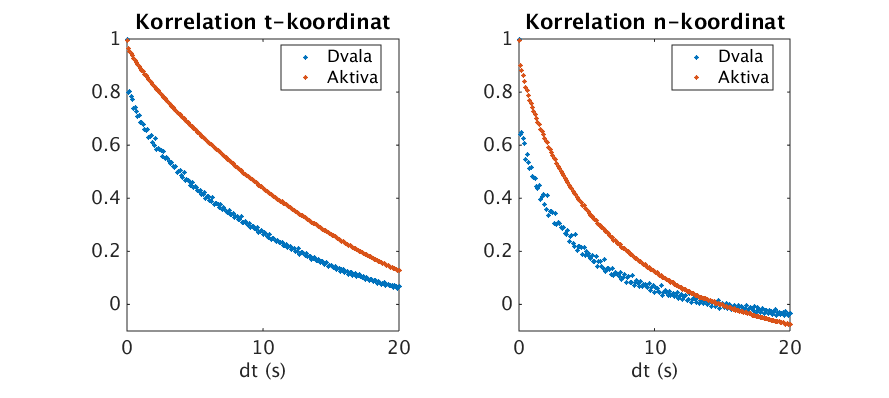
\includegraphics[width=.8\textwidth]{Korrelation_tnkoordinat.png}
    \caption{Korrelation i tangent- och normal-koordinaterna för aktiva celler och celler i dvala. I båda fall sjunker korrelationen initialt snabbare för cellerna i dvala. Korrelationen tycks även bestå längre i tangentialkoordinaten än normalkoordinaten vilket tyder på att det finns en föredragen väg.}
    \label{fig:Korr_tn}
\end{figure}

\paragraph{Avvikelse från brownsk rörelse}
%Har vi exempel på avvikelse från teorin kan dessa läggas under seprata underrubriker här
Utifrån teorin kring brownsk rörelse kan vissa förutsägelser göras för partiklar som strikt följer denna typ av rörelse. Bland annat räknades det fram i sektion \ref{sec:Brownsk} att mean square displacement (MSD) för en sådan partikel skulle öka linjärt med tiden, se ekvation \eqref{eq:MSD_Brownsk}. Utifrån givna data för arbetet har ett potenssamband kunnat anpassas med en exponent som är skilld från och betydligt lägre än 1. Detta tyder på att partikeln inte utför en ren brownsk rörelse utan genomgår en så kallad subdiffusion, karakteriserat att partikelns MSD beror av tiden via ett potenssamband med exponent mindre än 1 men större än 0.
\todo{Här kan bild infogas}

Vidare finns det minst två sätt att beräkna partiklarnas MSD. För stationära processer, dvs processer som inte explicit beror på när i tiden de inleds, kan man skapa ett medelvärde mellan alla möjliga mätpunkter separerade med givet tidsintervall så som beskrivet i ekvation ...
\todo{Kanske bör vi lägga till ett stycke om hur egenskaperna beräknas utifrån diskret data}
Genom att jämföra resultatet från denna typ av beräkning med att istället bara ta medelvärdet mellan alla partiklars kvadrerade radiella avvikelse från startpunkten vid given tid från start kan man avgöra om processen är stationär.
\todo{Bild för jämförelse mellan lilla och stora delta}
Båda dessa beräkningar har utförts för given data och exponentens värde i sambandet mellan MSD och tid skiljer sig/överensstämmer för lite för att någon tydlig slutsats hurvida processen är stationär eller ej ska kunna dras. \todo{Eller?}


\section{Diskussion och slutsats}







%Bara en liten kodsnutt som behövs när man kompilerar lokalt
%%% Local Variables: 
%%% mode: latex
%%% TeX-master: "main.tex"
%%% End: 

\chapter{Strängars rörelse i vätskor}

Bakgrund
\begin{itemize}
    \item WLC model, ev annan modell (Måns)
    \item Protein-filament
    \item Korrelationer, tangent, tid, rum
    \item Egenmoder
\end{itemize}

Resultat som kan tas med
\begin{itemize}
    \item Uppdelningen i egenmoder, olika relaxationstid
    \item Dispersionsrelation?
    \item Skillnad mellan confined och unconfined
    
\end{itemize}


\section{Teori}

\subsection{Proteinfilament}

Aktinfilament består av glubulära aktinprotein formade som bollar vilka kopplats ihop till en lång kedja.

\subsection{Modeller för strängrörelser}

\subsubsection{Worm Like Chain-model}

\subsubsection{Månsmodell}


\subsection{Egenomder}


\subsection{Lösning arv stokastisk differentialekvation}



\section{Tillhandahållen data}

Datan som analyserats i denna andra del av arbetet kommer från \todo{Var kommer datan från?}... och består av filmer av aktinfilament som tilåts röra sig i en vätska. Dessa strängar hade en storlek kring 10--30\,\micro{m} och befann sig i kanaler av olika bredd. Datan hade redan behandlats något så att strängens läge kunde beskrivas genom lägena för ett antal punker på strängen vilka angivna som pixlar i ett koordinatsystem. Genom att bildförstoringen och kamerans pixelstorlek var känd kunde de olika strängarnas längd beräknas. Mätningarna hade utförst på två ''fria'' strängar (strängar i breda skåror) och två strängar instängda i smala skåror, alla fyra filmade med 10 bilder per sekund. Rörelsen utfördes till största del i två dimensioner då skårornas djup var litet i förhållande till skårornas och filamentens bredd.

\section{Resultat}



\section{Diskussion och slutsats}





%Bara en liten kodsnutt som behövs när man kompilerar lokalt
%%% Local Variables: 
%%% mode: latex
%%% TeX-master: "main.tex"
%%% End: 








%%%%%%%%%%%%%%%%%%%%%%%%% Källförteckning %%%%%%%%%%%%%%%%%%%%%%%%%
\newpage
%Ser till att det blir rätt namn i rubriken
\iflanguage{swedish}{\renewcommand{\bibname}{Källförteckning}}{}
\bibliographystyle{babunsrt}
\bibliography{referenser_kandidat}%kräver en fil som heter 'referenser.bib'          

%%%%%%%%%%%%%%%%%%%%%%%%%%%%% Bilagor %%%%%%%%%%%%%%%%%%%%%%%%%%%%%
\clearpage
\appendix%Resets the section counter and changes it to Alph                 
\setcounter{page}{1} %Resets the pgenumbering                               
\renewcommand*{\thepage}{A\arabic{page}}%Changes the pagenubering to 'A...'
%Ser till at det blir rätt namn
\iflanguage{swedish}{\renewcommand{\appendixname}{Bilagor}}{}
\phantomsection{}%This one is needed to make 'Appendix' show up in the TOC
\addcontentsline{toc}{part}{\appendixname} %Makes 'Appendix' show up in the TOC
%Byter tillbaks till det gamla namnet
\iflanguage{swedish}{\renewcommand{\appendixname}{Bilaga}}{}




\end{document}





%% På svenska ska citattecknet vara samma i både början och slut.
%% Använd två apostrofer (två enkelfjongar): ''.

%% Inkludera PDF-dokument
\includepdf[pages={1-}]{filnamn.pdf} %Filnamnet får INTE innehålla 'mellanslag'!

%% Figurer inkluderade som pdf-filer
\begin{figure}\centering
\centerline{ %centrerar även större bilder
\includegraphics[width=1\textwidth]{filnamn.pdf}
}
\caption{\label{fig:} }
\end{figure}

%% Figurer inkluderade med xfigs "Combined PDF/LaTeX"
\begin{figure}\centering
\resizebox{.8\textwidth}{!}{\input{filnamn.pdf_t}}
\caption{\label{fig:} }
\end{figure}

%% Figurer roterade 90 grader
\begin{sidewaysfigure}\centering
\centerline{ %centrerar även större bilder
\includegraphics[width=1\textwidth]{filnamn.pdf}
}
\caption{\label{fig:} }
\end{sidewaysfigure}


%%Om man vill lägga till något i TOC
\stepcounter{section} %Till exempel en 'section'
\addcontentsline{toc}{section}{\Alph{section}\hspace{8 pt}Labblogg} 

